\documentclass[11pt,a4paper]{article}

\usepackage[T1]{fontenc}
\usepackage[utf8]{inputenc}
\usepackage{lmodern}
\usepackage{microtype}
\usepackage[margin=2.5cm]{geometry}
\usepackage{amsmath,amssymb}
\usepackage{booktabs,tabularx}
\usepackage[group-separator={,},group-minimum-digits=4]{siunitx}
\usepackage{xcolor}
\usepackage{pgfplots}
\pgfplotsset{compat=1.18}
\usepackage[font=small,labelfont=bf]{caption}
\usepackage[numbers,sort&compress]{natbib}
\usepackage[colorlinks=true,linkcolor=teal!70!black,citecolor=teal!70!black,urlcolor=teal!70!black]{hyperref}
\usepackage{cleveref}

\definecolor{sOne}{HTML}{2A78D6}
\definecolor{sTwo}{HTML}{EB6834}
\definecolor{sThree}{HTML}{1BAF7A}
\definecolor{accent}{HTML}{0F6E74}
\definecolor{neutral}{HTML}{8A9196}

\newcommand{\ioVol}{\iota_j}
\newcommand{\tauIO}{\tau^{\mathrm{IO}}}
\newcommand{\kapIO}{\kappa^{\mathrm{IO}}}
\newcommand{\code}[1]{\texttt{#1}}

\title{Result-data volume, egress price and transfer time\\for the FedHPC generated instances}
\author{FedHPC project --- methodology note}
\date{29 October 2026}

\begin{document}
\maketitle

\begin{abstract}
The FedHPC scheduling formulation charges each cloud-run job for the data it must
bring home (volume $\ioVol$, egress price $\kapIO_m$) and for the time that
transfer keeps the virtual machine busy ($\tauIO_m$). The Slurm logs behind the
two workloads record no I/O, so this note builds the three parameters from external
evidence: job-level Darshan I/O logs from two production machines, an I/O benchmark
of open reservoir-simulation decks under OPM Flow, the providers' price lists and
bandwidth documentation, and the literature on workload modelling and wide-area
transfer performance. An out-of-sample test on \num{140306} Theta jobs selects a
class-intercept, shared-slope power law in cores and runtime (test $R^2=0.52$,
against $-0.33$ for size and time alone). Its intercepts are three measured
output-retention policies of 0.02, 0.13 and \SI{1.5}{GB} per core-hour. A global
three-level scenario factor shifts the policies, which brackets the
0.48\,GB/core-h Azure-vs-AWS break-even. Transfer time follows the
minimum-of-subsystems model of \citet{liu2017explaining} and is bound by the cloud
disk's included throughput: \SI{7.63}{s/GB} on AWS and \SI{8.0}{s/GB} on Azure.
The purpose is to exercise every term of the weighted-sum formulation on realistic
magnitudes, not to forecast one site's I/O.
\end{abstract}

\section{Where I/O enters the formulation}\label{sec:formulation}
For job $j$ with execution time $e_j$ (slots) on instance type $m$ with relative
performance $P_m$ and deploy delay $\pi_m$, the formulation uses
\begin{align}
  p^{\mathrm{bill}}_{jm} &= e_j / P_m + \tauIO_m\, \ioVol, \label{eq:pbill}\\
  p^{\mathrm{occ}}_{jm}  &= \max\bigl(1, \lceil p^{\mathrm{bill}}_{jm} + \pi_m \rceil\bigr), \label{eq:pocc}\\
  c_{jm} &= \kapIO_m\, \ioVol + \kappa^{\mathrm{VM}}_m\, p^{\mathrm{bill}}_{jm}
           + \kappa^{\mathrm{S}}_m\, q^{\mathrm{stor}}_j\, p^{\mathrm{bill}}_{jm}. \label{eq:cost}
\end{align}
Earlier generated instances had $\ioVol=\tauIO_m=\kapIO_m=0$, so these terms
were never exercised. With them set, data movement enters both objectives. Cost
($f_2$) grows through egress and through the VM time billed while the upload runs.
Turnaround ($f_1$) grows because a cloud job holds its slot until its results are
home. On-prem types keep $\tauIO_m=\kapIO_m=0$, because results written there are
already where the user needs them.

\section{Approach: model plus scenario factor}\label{sec:approach}
Both workloads, \code{fedhpc} (964 jobs) and \code{pos} (\num{3340} jobs), come
from the site's Slurm accounting. It records cores, memory, elapsed time, job
name and working directory, but no bytes. Since there is no per-job ground truth
to fit, the approach has two parts:
\begin{enumerate}
  \item a \emph{volume model} whose form and spread come from the I/O literature
        and job-level Darshan logs, with intercepts calibrated on open reservoir
        simulations; and
  \item a \emph{scenario factor} (io level L/M/H) that shifts the intercepts across
        the range the evidence supports, so results can be read as a sensitivity
        analysis \citep{feitelson2015workload}.
\end{enumerate}
A single global average was ruled out. Per-job output in production spans more
than ten decades (\cref{tab:darshan}), so an average would give every job a
volume that almost no job actually has.

\section{Evidence}\label{sec:evidence}
\subsection{Job-level I/O on production machines}
Darshan \citep{carns2011understanding} records POSIX and STDIO byte counters per job.
The Darshan data page and the facility portals sit behind interactive gates, so
the two public Zenodo releases were used. ALCF Theta 2017--2020
\citep{alcf2021theta} has \num{439367} jobs over 412 anonymised applications.
NERSC Cori, April 2019 \citep{bez2022access}, has \num{73857} jobs tagged with
the project's science domain; it is licensed CC BY-NC-ND~4.0, so only aggregates
are reported here. The target is bytes written to files that were written but
never read back, a proxy for result data.

\begin{table}[ht]
\centering\small
\caption{Per-job output volume. On Theta, which application a job ran explains
64\,\% of the variance of $\log_{10}$ output.}\label{tab:darshan}
\begin{tabular}{lrrrrr}
\toprule
Population & Jobs & Zero output & Median & p90 & p99 \\
\midrule
Theta, write-only bytes & \num{439367} & 48\,\% & $\approx$\SI{1}{KB} & \SI{0.61}{GB} & \SI{687}{GB} \\
Cori, all bytes written & \num{73857}  & 1\,\%  & \SI{58}{MB}  & \SI{3.0}{GB} & \SI{235}{GB} \\
Cori, Energy Sciences   & \num{2358}   & 0\,\%  & \SI{85}{MB}  & \SI{5.1}{GB} & \SI{24}{GB}  \\
Cori, Earth Science     & 976          & 0.1\,\%& \SI{0.62}{GB}& \SI{167}{GB} & \SI{167}{GB} \\
\bottomrule
\end{tabular}
\end{table}

\subsection{Reservoir-simulation output, measured}
The site's job names point to reservoir studies (history matching, optimisation,
uncertainty analysis), mostly as ensembles of one deck. Open decks were run in
OPM Flow 2026.04 \citep{rasmussen2021opm} instrumented with Darshan~3.5.0 in a
container: SPE1/3/5/9 \citep{killough1995ninth}, SPE10 \citep{christie2001tenth},
Norne \citep{rwechungura2010norne}, Drogon, Model~2 and UNISIM-I-D
\citep{avansi2015unisim}; the last had no schedule, so a 30-year forecast was
appended. Output was split by Eclipse file type into three retention policies:
\textbf{S}, summary vectors only (UNSMRY, SMSPEC, ESMRY);
\textbf{R}, summary plus grid, initial state and a final restart (UNISIM-I-D as
shipped); and \textbf{F}, a restart record at every report step (Norne, Drogon
and SPE10 as shipped, or UNISIM with \code{RPTRST BASIC=2}). Restart volume is set
by the deck's \code{RPTRST} keyword: OPM's command-line output flags produced
byte-identical files.

\begin{figure}[ht]
\centering
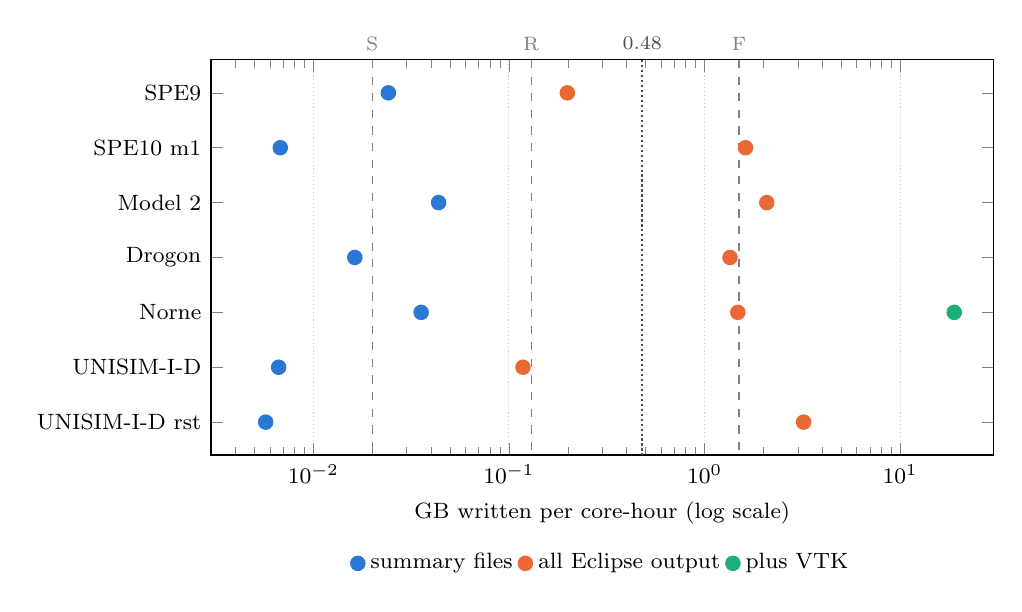
\begin{tikzpicture}
\begin{axis}[
  width=0.95\linewidth, height=6.6cm, xmode=log, xmin=0.003, xmax=30,
  ytick={1,...,7}, yticklabels={SPE9,SPE10 m1,Model 2,Drogon,Norne,UNISIM-I-D,UNISIM-I-D rst},
  y dir=reverse, ymin=0.4, ymax=7.6, xlabel={GB written per core-hour (log scale)},
  tick label style={font=\footnotesize}, label style={font=\footnotesize},
  xmajorgrids, grid style={densely dotted, gray!40},
  legend style={font=\footnotesize, draw=none, at={(0.5,-0.22)}, anchor=north, legend columns=3},
  clip=false]
\addplot[only marks, mark=*, mark size=2.6pt, color=sOne] coordinates
  {(0.0242,1) (0.00678,2) (0.0437,3) (0.0163,4) (0.0356,5) (0.00665,6) (0.00571,7)};
\addlegendentry{summary files}
\addplot[only marks, mark=*, mark size=2.6pt, color=sTwo] coordinates
  {(0.199,1) (1.62,2) (2.08,3) (1.35,4) (1.48,5) (0.118,6) (3.21,7)};
\addlegendentry{all Eclipse output}
\addplot[only marks, mark=*, mark size=2.6pt, color=sThree] coordinates {(18.9,5)};
\addlegendentry{plus VTK}
\draw[gray, dashed] (axis cs:0.02,0.4) -- (axis cs:0.02,7.6) node[pos=0, above, font=\scriptsize] {S};
\draw[gray, dashed] (axis cs:0.13,0.4) -- (axis cs:0.13,7.6) node[pos=0, above, font=\scriptsize] {R};
\draw[gray, dashed] (axis cs:1.5,0.4) -- (axis cs:1.5,7.6) node[pos=0, above, font=\scriptsize] {F};
\draw[black!70, densely dotted, thick] (axis cs:0.48,0.4) -- (axis cs:0.48,7.6)
  node[pos=0, above, font=\scriptsize] {0.48};
\end{axis}
\end{tikzpicture}
\caption{Output per core-hour of each OPM run (core-hours = wall time $\times$ 2
threads). Summary output stays near 0.02\,GB/core-h on every deck. Full
output lies between 0.1 and 3.2 depending on restart frequency. Dashed lines mark
the policy rates, the dotted line the Azure break-even of \cref{sec:price}.}
\label{fig:rates}
\end{figure}

\begin{table}[ht]
\centering\small
\caption{OPM runs: output rate and egress relative to compute, at AWS egress
\$0.090/GB and compute \$0.096 per core-hour (m6i.24xlarge, \$4.608/h over 48
physical cores).}\label{tab:opm}
\begin{tabular}{lrrrrr}
\toprule
& & \multicolumn{2}{c}{GB per core-hour} & \multicolumn{2}{c}{Egress / compute} \\
\cmidrule(lr){3-4}\cmidrule(lr){5-6}
Case & Active cells & summary & all Eclipse & summary & all \\
\midrule
SPE9                        & \num{9000}  & 0.024 & 0.20 & 2.3\,\% & 19\,\% \\
SPE10 model 1               & \num{2000}  & 0.007 & 1.62 & 0.6\,\% & 152\,\% \\
Model 2                     & \num{2794}  & 0.044 & 2.08 & 4.1\,\% & 195\,\% \\
Drogon                      & \num{70972} & 0.016 & 1.35 & 1.5\,\% & 127\,\% \\
Norne                       & \num{44431} & 0.036 & 1.48 & 3.3\,\% & 138\,\% \\
UNISIM-I-D, as shipped      & \num{36403} & 0.007 & 0.12 & 0.6\,\% & 11\,\% \\
UNISIM-I-D, restart every step & \num{36403} & 0.006 & 3.21 & 0.5\,\% & 301\,\% \\
Norne + VTK                 & \num{44431} & 0.043 & 18.9\textsuperscript{a} & 4.0\,\% & 1774\,\% \\
\bottomrule
\multicolumn{6}{l}{\footnotesize \textsuperscript{a} including \SI{3.1}{GB} of VTK visualisation files.}
\end{tabular}
\end{table}

\section{Model selection}\label{sec:selection}
Workload-modelling and I/O-characterisation work offers four families of volume
model: a single fitted distribution \citep{feitelson2015workload}; a function of
correlated job attributes such as size and runtime, in the spirit of
\citet{lublin2003workload}; class or application-level models
\citep{feitelson2015workload,luu2015multiplatform}; and learned models over Darshan
counters \citep{isakov2020hpc}, which need counters this setting does not have. The
first three, plus their combination, were compared on the Theta jobs that ran at
least 10~minutes (\num{140306} jobs, 214 applications). The target was
$\log_{10}$ write-only bytes of jobs that wrote something. Training used the first
75\,\% of jobs by start time and testing the last 25\,\% (split on 15 June 2019),
so no model learns from the future.

\begin{table}[ht]
\centering\small
\caption{Out-of-sample fit on Theta. 26\,\% of test jobs come from applications
unseen in training; M2--M4 fall back to M1 for them.}\label{tab:models}
\begin{tabularx}{\linewidth}{lXrr}
\toprule
Model & Form & Test $R^2$ & RMSE (decades) \\
\midrule
M0 & global mean & $-0.09$ & 2.52 \\
M1 & $a + b\log c_j + d\log h_j$ (pooled power law) & $-0.33$ & 2.78 \\
M2 & class mean & 0.57 & 1.59 \\
\textbf{M3} & \textbf{class intercept + shared $b, d$ (ANCOVA)} & \textbf{0.52} & \textbf{1.67} \\
M4 & class-specific $b, d$ ($\geq 30$ training jobs, else M3) & 0.66 & 1.41 \\
\bottomrule
\end{tabularx}
\end{table}

Pooled, M1's exponents are 1.09 for cores and 2.01 for runtime. Within classes they
fall to 0.54 and 1.05: pooled size and time mostly stand in for which application
ran. M3 was chosen over M4 although M4 scores higher, because the instance
workloads carry no I/O data from which to estimate per-class slopes. M3 separates
what transfers from what does not. The intercept is the measured output policy of
the job's class (\cref{sec:evidence}), and the scaling in size and time is shared,
so it can be taken from Theta.

The zero-output part of a two-part (hurdle) model \citep{cragg1971some} was left out.
A class-rate predictor of zero output was worse than the global rate out of sample
(Brier score 0.356 against 0.333), the zero share drifted between periods, and a
reservoir run always writes its summary vectors.

\section{The volume model}\label{sec:volume}
\begin{equation}
  \ioVol = r(\text{policy}_j)\; c_{\mathrm{ref}}\,
  \Bigl(\frac{c_j}{c_{\mathrm{ref}}}\Bigr)^{\beta_p} h_j^{\beta_t}\; 10^{\sigma z_j}
  \quad\text{[GB]},
  \label{eq:volume}
\end{equation}
where $c_j$ is the job's core count and $h_j$ its runtime in hours.

\begin{table}[ht]
\centering\small
\caption{Parameters of \cref{eq:volume}.}\label{tab:params}
\begin{tabularx}{\linewidth}{llX}
\toprule
Term & Value & Source and reasoning \\
\midrule
$r(\mathrm{S}), r(\mathrm{R}), r(\mathrm{F})$ & 0.02, 0.13, 1.5 GB/core-h &
  Median of the OPM runs per policy (\cref{fig:rates}). $r$ is the median volume;
  the noise lifts the mean by $\exp\bigl((\sigma\ln 10)^2/2\bigr)\approx 1.9$. \\
$\beta_t$ & 1 & Output records grow with simulated time, which grows with wall time
  at fixed cells per core; Theta's within-class fit is 1.05. \\
$\beta_p$ & 0.54 & Theta within-class fit (weak scaling would give 1). Jobs here
  span 1--64 cores, so the choice moves volumes by at most 0.85 decades. \\
$c_{\mathrm{ref}}$ & 40 cores & Modal job size in both workloads. \\
$\sigma$ & 0.5 decades & Median within-class spread on Theta (interquartile range
  0.09--1.15). \\
$z_j$ & $\mathcal N(0,1)$, clipped to $\pm 3$ & One draw per (workload, job), seeded
  by hash and reused at every level (common random numbers \citep{law2015simulation}),
  so volumes are nested across levels. \\
\bottomrule
\end{tabularx}
\end{table}

\paragraph{Classes.} A job is an \emph{ensemble member} when at least 10 jobs of
its workload share its (user, job-name stem), the stem being the name with trailing
run numbers removed. Otherwise it is a \emph{single run}. This gives 945 of 964
ensemble jobs in \code{fedhpc} (98\,\%) and \num{3194} of \num{3340} in \code{pos}
(96\,\%), consistent with ensemble-based history matching and optimisation
\citep{oliver2011recent}. Only the 0/1 labels are stored
(\code{data/job\_classes\_*.json}).

\paragraph{Io levels.} With most jobs in ensembles, a rule like ``ensembles keep
summaries only'' would make two levels nearly identical. Each level therefore moves
both classes up one policy (\cref{tab:levels}).

\begin{table}[ht]
\centering\small
\caption{Io levels and the data they imply if every job ran in the cloud.}\label{tab:levels}
\begin{tabular}{llllrrr}
\toprule
Level & Ensemble & Single run & Reading & \code{fedhpc} & \code{pos} & Median job \\
\midrule
L & S & R & only curves return       & \SI{2.6}{TB} & \SI{16}{TB}  & \SI{0.4}{GB} \\
M & R & F & decks as typically shipped & \SI{21}{TB}  & \SI{147}{TB} & 2.4--\SI{2.9}{GB} \\
H & F & F & full restart history      & \SI{142}{TB} & \SI{640}{TB} & 26--\SI{33}{GB} \\
\bottomrule
\end{tabular}
\end{table}

\paragraph{Horizon guard.} A volume is capped where its transfer would push the
job's cloud completion past the horizon $H$ even from its release slot $r_j$, i.e.\
$\ioVol \le (H - r_j - e_j)/\max_m \tauIO_m$. Every cloud option then stays
feasible. This affects no \code{fedhpc} job and 3 (M) or 7 (H) of \num{3340}
\code{pos} jobs.

\section{Egress price}\label{sec:price}
Prices come from the providers' machine-readable lists: the AWS Price List API
(AWSDataTransfer, us-east-1, publication 16 September 2026) and the Azure Retail
Prices API (Bandwidth, eastus). The first paid tier of internet egress is used:
\$0.090/GB on AWS and \$0.080/GB on Azure with \emph{routing preference: internet},
i.e.\ ISP transit as on AWS (\$0.087 over Microsoft's network). Volume tiers and
the free \SI{100}{GB} per month are ignored. The cloud equivalents have the same
on-demand price on both providers except at 128 vCPU: Standard\_D128s\_v6 costs
\$6.451/h against \$6.144/h for m6i.32xlarge. For a 64-core job, Azure's dearer VM
is paid back by its cheaper egress once the job writes
\begin{equation}
  \frac{(6.451-6.144)/64}{0.090-0.080} = \frac{0.0048}{0.010}
  = 0.48\ \text{GB per core-hour},
\end{equation}
which lies between the L and H rates. At every other size, any output makes Azure
cheaper.

\section{Transfer time}\label{sec:transfer}
\citet{liu2017explaining} bound the achievable rate of an end-to-end transfer by its
slowest subsystem,
\begin{equation}
  R_{\max} \le \min\bigl(DR_{\max},\, MM_{\max},\, DW_{\max}\bigr),
\end{equation}
where $DR$ is the source disk read, $MM$ the memory-to-memory network path and $DW$
the sink disk write. They validated this on ESnet testbed transfers and on Globus
logs. Each term was filled from provider documentation (\cref{tab:bottleneck}).
Skyplane \citep{jain2023skyplane} independently measured the same egress caps:
AWS throttles egress at \SI{5}{Gbps}, and Azure has no limit beyond the VM's own.

\begin{table}[ht]
\centering\small
\caption{Rate limits of a result upload. The included disk throughput binds on both
providers.}\label{tab:bottleneck}
\begin{tabularx}{\linewidth}{lXX}
\toprule
Subsystem & AWS & Azure \\
\midrule
Source disk (binds) & EBS gp3 baseline included in price, 125\,MiB/s = \SI{131}{MB/s} \citep{aws-ebs} &
  Premium SSD v2 baseline included in price, \SI{125}{MB/s} \citep{azure-disks} \\
Network & Internet-gateway traffic: \SI{5}{Gbps} below 32 vCPU, else 50\,\% of instance
  bandwidth (m6i 8--32xlarge: 12.5--\SI{50}{Gbps}); single flow \SI{5}{Gbps}
  \citep{aws-bandwidth,aws-gp} &
  All egress counts toward VM bandwidth, any destination (Dsv5/Dsv6: 16--\SI{54}{Gbps})
  \citep{azure-bandwidth,azure-sizes} \\
Sink & \multicolumn{2}{l}{On-prem parallel file system, not binding at one stream} \\
\bottomrule
\end{tabularx}
\end{table}

\begin{figure}[ht]
\centering
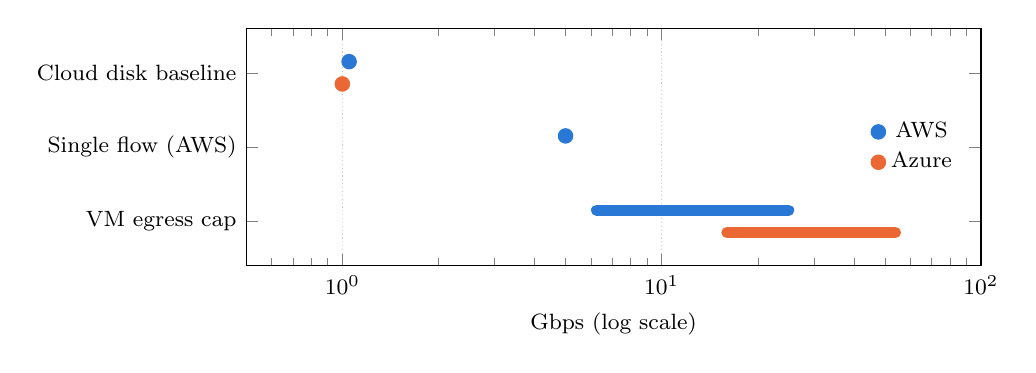
\begin{tikzpicture}
\begin{axis}[
  width=0.9\linewidth, height=4.6cm, xmode=log, xmin=0.5, xmax=100,
  ytick={1,2,3}, yticklabels={Cloud disk baseline, Single flow (AWS), VM egress cap},
  y dir=reverse, ymin=0.4, ymax=3.6, xlabel={Gbps (log scale)},
  tick label style={font=\footnotesize}, label style={font=\footnotesize},
  xmajorgrids, grid style={densely dotted, gray!40},
  legend style={font=\footnotesize, draw=none, at={(0.98,0.5)}, anchor=east}]
\addplot[only marks, mark=*, mark size=2.6pt, color=sOne] coordinates {(1.05,0.85) (5,1.85)};
\addlegendentry{AWS}
\addplot[only marks, mark=*, mark size=2.6pt, color=sTwo] coordinates {(1.0,1.15)};
\addlegendentry{Azure}
\draw[sOne, line width=4pt, line cap=round] (axis cs:6.25,2.85) -- (axis cs:25,2.85);
\draw[sTwo, line width=4pt, line cap=round] (axis cs:16,3.15) -- (axis cs:54,3.15);
\end{axis}
\end{tikzpicture}
\caption{Rate limit per subsystem, smallest to largest VM in the catalogue. The disk
baseline is the minimum on both providers.}
\label{fig:bottleneck}
\end{figure}

With 600-second slots,
\begin{align}
  \tauIO_{\mathrm{AWS}}   &= \frac{1000}{131.07 \cdot 600} = 0.0127\ \text{slot/GB}\quad(\SI{7.63}{s/GB}),\\
  \tauIO_{\mathrm{Azure}} &= \frac{1000}{125 \cdot 600} = 0.0133\ \text{slot/GB}\quad(\SI{8.0}{s/GB}).
\end{align}
The two providers end up nearly equal, as two clouds on common internet routing
would be. The 5\,\% difference comes straight from the documented baselines, and it
makes Azure the cheaper but slightly slower egress, so neither provider dominates
the other in both objectives. A faster disk could be provisioned, but storage
performance is not priced in the formulation ($\kappa^{\mathrm S}=0$), so the
default tier is the consistent choice.

\section{Instance design}\label{sec:design}
An instance is named by its factors and rebuilt bit for bit from the name. Node
counts take 100/300/500 per on-prem type. Initial load (F free, H half, E full) and
io level (L/M/H) each take one value for the whole instance; one value per type
would multiply the space beyond what can be covered at every io level. Class~A
(c40, c64 + AWS) has 162 distinct instances, all benchmarked. Class~B (c32, c40,
c64, m32, plus c16 in \code{pos}, each with an AWS and an Azure equivalent) has
\num{1944} distinct instances, down from \num{36450} with load per type. Its
benchmark set is a strength-2 orthogonal array over the $k+2$ three-level factors
(Rao--Hamming construction \citep{hedayat1999orthogonal}) plus the 27 uniform
corners: 104 instances. Types that fit exactly the same jobs are collapsed to a
canonical order.

Running-job draws are nested across loads (the half-full set is a prefix of the full
one), and volumes are nested across io levels. Optimal turnaround and optimal cost
can therefore only grow along a load chain $\mathrm F\to\mathrm H\to\mathrm E$ or an
io chain $\mathrm L\to\mathrm M\to\mathrm H$. Greedy earliest-completion always lies
between ``every job at release on its fastest type'' and ``every job at release in
the cloud''. The test suite checks all of these with exact Gurobi solves. The
space-time dominance reductions stay exact with type-dependent occupation, because
they compare options per (job, type).

\section{Effect on the instances}\label{sec:effect}
\begin{table}[ht]
\centering\small
\caption{Class B at load E, per job: cheapest Azure option against cheapest AWS
option, and the cloud's added occupancy over the on-prem run time (600-s slots).}
\label{tab:effect}
\begin{tabular}{lrrrrr}
\toprule
Workload, level & Azure cheaper & AWS cheaper & Azure slower & Extra slots p90 & max \\
\midrule
\code{fedhpc}, L & 99\,\%  & 0\,\% & 0\,\% & 0 & 3 \\
\code{fedhpc}, M & 100\,\% & 0\,\% & 1\,\% & 1 & 31 \\
\code{fedhpc}, H & 100\,\% & 0\,\% & 9\,\% & 4 & 103 \\
\code{pos}, L    & 98\,\%  & 1\,\% & 0\,\% & 0 & 13 \\
\code{pos}, M    & 99\,\%  & 0\,\% & 2\,\% & 1 & 122 \\
\code{pos}, H    & 100\,\% & 0\,\% & 9\,\% & 4 & 138 \\
\bottomrule
\end{tabular}
\end{table}
AWS keeps its equal-price offer, and no quota is applied. It is now the dearer
provider for almost every job and is preferred only where turnaround weighs more
than cost, e.g.\ for the 9\,\% of jobs whose Azure option is slower at level H. This
is a genuine trade-off for the weighted sum to resolve, and it does not exist
without I/O.

\section{Limitations}\label{sec:limits}
Volumes are modelled, not observed; the io level expresses that uncertainty, so
results should be compared across levels. Exponents and spread come from Theta, a
different machine and application mix. Each job is assumed to upload alone at the
disk-bound rate: congestion on the site's WAN link is not modelled, because
$\tauIO_m$ is a per-type constant. Prices use the first paid tier, though a month
at level H would reach cheaper tiers. Ensemble detection by name stem is a
heuristic: threshold 10 keeps optimisation rounds of 10 runs inside the ensemble
class.

\begin{thebibliography}{99}\small
\bibitem[Cragg(1971)]{cragg1971some} J.~G. Cragg. Some statistical models for limited dependent variables with application to the demand for durable goods. \emph{Econometrica}, 39(5):829--844, 1971.
\bibitem[Feitelson(2015)]{feitelson2015workload} D.~G. Feitelson. \emph{Workload Modeling for Computer Systems Performance Evaluation}. Cambridge University Press, 2015.
\bibitem[Lublin and Feitelson(2003)]{lublin2003workload} U.~Lublin and D.~G. Feitelson. The workload on parallel supercomputers: modeling the characteristics of rigid jobs. \emph{J. Parallel Distrib. Comput.}, 63(11):1105--1122, 2003.
\bibitem[Carns et~al.(2011)]{carns2011understanding} P.~Carns et~al. Understanding and improving computational science storage access through continuous characterization. \emph{ACM Trans. Storage}, 7(3), 2011.
\bibitem[Luu et~al.(2015)]{luu2015multiplatform} H.~Luu et~al. A multiplatform study of I/O behavior on petascale supercomputers. In \emph{Proc. HPDC}, 2015.
\bibitem[Bez et~al.(2022)]{bez2022access} J.~L. Bez et~al. Access patterns and performance behaviors of multi-layer supercomputer I/O subsystems under production load. In \emph{Proc. HPDC}, 2022. Dataset: Zenodo 6476501, CC BY-NC-ND~4.0.
\bibitem[ALCF(2021)]{alcf2021theta} Argonne Leadership Computing Facility. Darshan job summaries, Theta 2017--2020. Zenodo 4902920.
\bibitem[Isakov et~al.(2020)]{isakov2020hpc} M.~Isakov et~al. HPC I/O throughput bottleneck analysis with explainable local models. In \emph{Proc. SC}, 2020.
\bibitem[Liu et~al.(2017)]{liu2017explaining} Z.~Liu, P.~Balaprakash, R.~Kettimuthu, and I.~Foster. Explaining wide area data transfer performance. In \emph{Proc. HPDC}, pages 167--178, 2017.
\bibitem[Jain et~al.(2023)]{jain2023skyplane} P.~Jain, S.~Kumar, S.~Wooders, S.~G. Patil, J.~E. Gonzalez, and I.~Stoica. Skyplane: optimizing transfer cost and throughput using cloud-aware overlays. In \emph{Proc. NSDI}, 2023. arXiv:2210.07259.
\bibitem[Hedayat et~al.(1999)]{hedayat1999orthogonal} A.~S. Hedayat, N.~J.~A. Sloane, and J.~Stufken. \emph{Orthogonal Arrays: Theory and Applications}. Springer, 1999.
\bibitem[Law(2015)]{law2015simulation} A.~M. Law. \emph{Simulation Modeling and Analysis}, 5th ed. McGraw-Hill, 2015.
\bibitem[Rasmussen et~al.(2021)]{rasmussen2021opm} A.~F. Rasmussen et~al. The Open Porous Media Flow reservoir simulator. \emph{Comput. Math. Appl.}, 81:159--185, 2021.
\bibitem[Christie and Blunt(2001)]{christie2001tenth} M.~A. Christie and M.~J. Blunt. Tenth SPE comparative solution project: a comparison of upscaling techniques. \emph{SPE Reserv. Eval. Eng.}, 4(4):308--317, 2001.
\bibitem[Killough(1995)]{killough1995ninth} J.~E. Killough. Ninth SPE comparative solution project: a reexamination of black-oil simulation. SPE 29110, 1995.
\bibitem[Rwechungura et~al.(2010)]{rwechungura2010norne} R.~Rwechungura et~al. The Norne field case: a unique comparative case study. SPE 127538, 2010.
\bibitem[Avansi and Schiozer(2015)]{avansi2015unisim} G.~D. Avansi and D.~J. Schiozer. UNISIM-I: synthetic model for reservoir development and management applications. \emph{Int. J. Model. Simul. Pet. Ind.}, 9(1), 2015.
\bibitem[Oliver and Chen(2011)]{oliver2011recent} D.~S. Oliver and Y.~Chen. Recent progress on reservoir history matching: a review. \emph{Comput. Geosci.}, 15:185--221, 2011.
\bibitem[AWS(2026a)]{aws-bandwidth} Amazon Web Services. Amazon EC2 instance network bandwidth. \url{https://docs.aws.amazon.com/AWSEC2/latest/UserGuide/ec2-instance-network-bandwidth.html}.
\bibitem[AWS(2026b)]{aws-gp} Amazon Web Services. Network specifications, general purpose instances. \url{https://docs.aws.amazon.com/ec2/latest/instancetypes/gp.html}.
\bibitem[AWS(2026c)]{aws-ebs} Amazon Web Services. Amazon EBS General Purpose SSD volumes. \url{https://docs.aws.amazon.com/ebs/latest/userguide/general-purpose.html}.
\bibitem[Microsoft(2026a)]{azure-disks} Microsoft. Azure managed disk types. \url{https://learn.microsoft.com/en-us/azure/virtual-machines/disks-types}.
\bibitem[Microsoft(2026b)]{azure-bandwidth} Microsoft. Virtual machine network bandwidth. \url{https://learn.microsoft.com/en-us/azure/virtual-network/virtual-machine-network-throughput}.
\bibitem[Microsoft(2026c)]{azure-sizes} Microsoft. Dsv5 and Dsv6 size series. \url{https://learn.microsoft.com/en-us/azure/virtual-machines/sizes/general-purpose/dsv5-series}, \url{https://learn.microsoft.com/en-us/azure/virtual-machines/sizes/general-purpose/dsv6-series}.
\end{thebibliography}

\end{document}
